\documentclass{beamer}
\usefonttheme{serif}
\title{Killer Yeast Vs. Sensitive Yeast}
\author{Evan Cummings \and Intizor Aliyorov \and Malachi J.\ Cryder\\
\vspace{5mm}
MATH 445 - Statistical, Dynamical, and Computational Modeling}
\begin{document}
\frame{\titlepage}

%% frame =======================================================================
\begin{frame}
  \frametitle{Experiment}
  An experiment was conducted where an amount of yeast was grown in \emph{chemostat} and allowed to come to equilibrium.  The steady-state \emph{optical density} of the yeast was recorded for a given flow rate $F$.
\end{frame}

%% frame =======================================================================
\begin{frame}
  \frametitle{Chemostat}
  \begin{figure}[H]
    \centering
      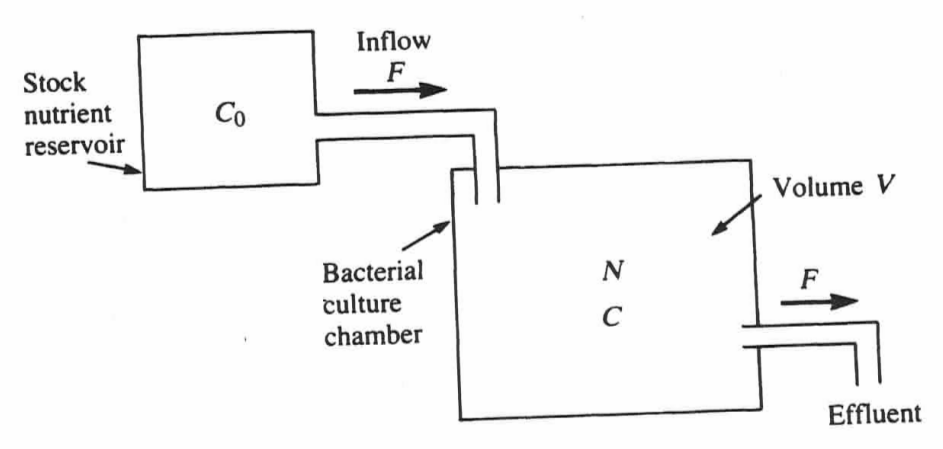
\includegraphics[width=1.0\textwidth]{images/chemostat.png}
  \end{figure}
\end{frame}

%% frame =======================================================================
\begin{frame}
  \frametitle{Optical Density}
  \begin{figure}[H]
    \centering
      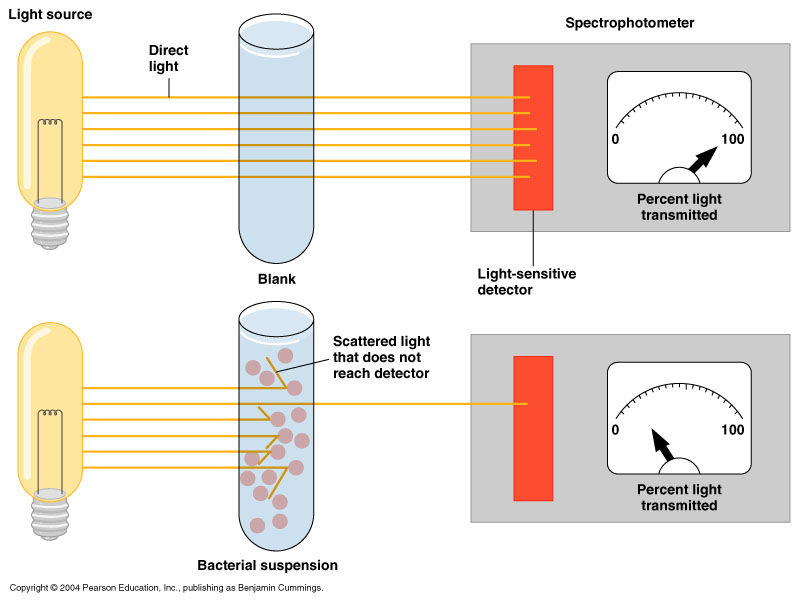
\includegraphics[width=0.8\textwidth]{images/optical_density.jpg}
  \end{figure}
\end{frame}

%% frame =======================================================================
\begin{frame}
  \frametitle{ODE}
  The differential equation we may use for modeling the growth of yeast is the same as that used for bacterial growth in a chemostat:
  \begin{align*}
    \frac{dN}{dt} &= k(C) N - \frac{FN}{V}, \\
    \frac{dC}{dt} &= -\alpha k(C) N - \frac{FC}{V} + \frac{FC_0}{V},
  \end{align*}
  with initial conditions $C(0) = C_i$ and $N(0) = N_i$, $N$ is the unitless optical density of yeast in the chamber, $C$ is the unitless optical density of nutrient in the chamber, $C_0$ is the unitless optical density of nutrient in the reservoir, $F$ is the in/out volume flow rate with units volume/time, $V$ is the volume of the chamber, $\alpha$ is a unitless inverse of the yield constant, and $k(C)$ is the reproduction rate for yeast in units 1/time.
\end{frame}

%% frame =======================================================================
\begin{frame}
  \frametitle{$k(C)$ and its Simplification}
  $k(C)$ is the reproduction rate for yeast in units 1/time with possible formula chosen such that $\lim_{C \rightarrow \infty} = k_{max}$, and $k_{max}$ represents the maximum possible reproduction rate:
  $$k(C) = \frac{k_{max} C}{C_n + C}.$$
  where $C_n$ is chosen such that $k(C_n) = k_{max} / 2$.  Because the concentration in the tank $C(t)$ is related to the concentration in the reservoir by $C(t) \leq C_0$, $C_0$ may be chosen sufficiently small such that 
  \begin{align*}
    k(C) = \frac{k_{max} C}{C_n + C} \approx \frac{k_{max} C}{C_n} = KC,
  \end{align*}
  with $K$ in units 1/time.
\end{frame}

%% frame =======================================================================
\begin{frame}
  \frametitle{New ODE}
  The equations we need to solve then become 
  \begin{align}
    \frac{dN}{dt} &= KCN - \frac{FN}{V}, \\
    \frac{dC}{dt} &= -\alpha KCN - \frac{FC}{V} + \frac{FC_0}{V}.
  \end{align}
\end{frame}

%% frame =======================================================================
\begin{frame}
  \frametitle{Steady States}
  The quantitative measurement for fitness is a unitless measurement of optical density at steady state ($N$) at a given flow rate ($F$) in volumes/hr.  In order to find the steady states, we have to find the intersections of the null-clines at equilibrium points $(\bar{N}, \bar{C})$, i.e.\ $dN(\bar{N},\bar{C})/dt = 0$ and $dC(\bar{N},\bar{C})/dt = 0$:
\end{frame}

%% frame =======================================================================
\begin{frame}
  \frametitle{$dN(\bar{N},\bar{C})/dt = 0$}
  \begin{align*}
    \frac{dN(\bar{N}, \bar{C})}{dt} &= K\bar{C} \bar{N} - \frac{F\bar{N}}{V}, \\
    &= \bar{N} \left( K\bar{C} - \frac{F}{V} \right) = 0, \\
  \end{align*}
  which is zero for $\bar{N} = 0$ or $K \bar{C} = F/V$.
\end{frame}

%% frame =======================================================================
\begin{frame}
  \frametitle{$dC(\bar{N},\bar{C})/dt = 0$}
  \begin{align*}
    \frac{dC(\bar{N}, \bar{C})}{dt} &= -\alpha K \bar{C} \bar{N} - \frac{F\bar{C}}{V} + \frac{FC_0}{V} = 0,
  \end{align*}
  which is zero for $\alpha K\bar{C} \bar{N} + \frac{F\bar{C}}{V} = \frac{FC_0}{V}$.
\end{frame}

%% frame =======================================================================
\begin{frame}
  \frametitle{Determination of $(\bar{N}, \bar{C})$}
  In order to evaluate these null-clines, we need to evaluate the non-trivial cases, here for $\dot{N} = 0$,
  \begin{align}
    K \bar{C} = \frac{F}{V} \implies \bar{C} = \frac{F}{VK}.
  \end{align}
  Likewise, for $\dot{C} = 0$,
  \begin{align}
    \alpha K \bar{C} \bar{N} + \frac{F\bar{C}}{V} &= \frac{FC_0}{V} \notag \\
    \implies \bar{N} &= \frac{FC_0}{V \alpha K \bar{C}} - \frac{F}{V \alpha K} = \frac{F}{V \alpha K} \left(\frac{C_0}{\bar{C}} - 1 \right).
  \end{align}
  This intersects the $\bar{N} = 0$ nullcline at $\frac{F}{V\alpha K} = 0$ or $\frac{C_0}{\bar{C}} = 1$.  However, because $F$ is never 0, we can disregard the first equation, and we know that the only trivial steady-state is located at $\bar{N} = 0$, $\bar{C} = C_0$.
\end{frame}

%% frame =======================================================================
\begin{frame}
  \frametitle{Determination of $(\bar{N}, \bar{C})$}
  \begin{columns}
  \begin{column}{0.4\textwidth}
  \begin{figure}[H]
    \centering
      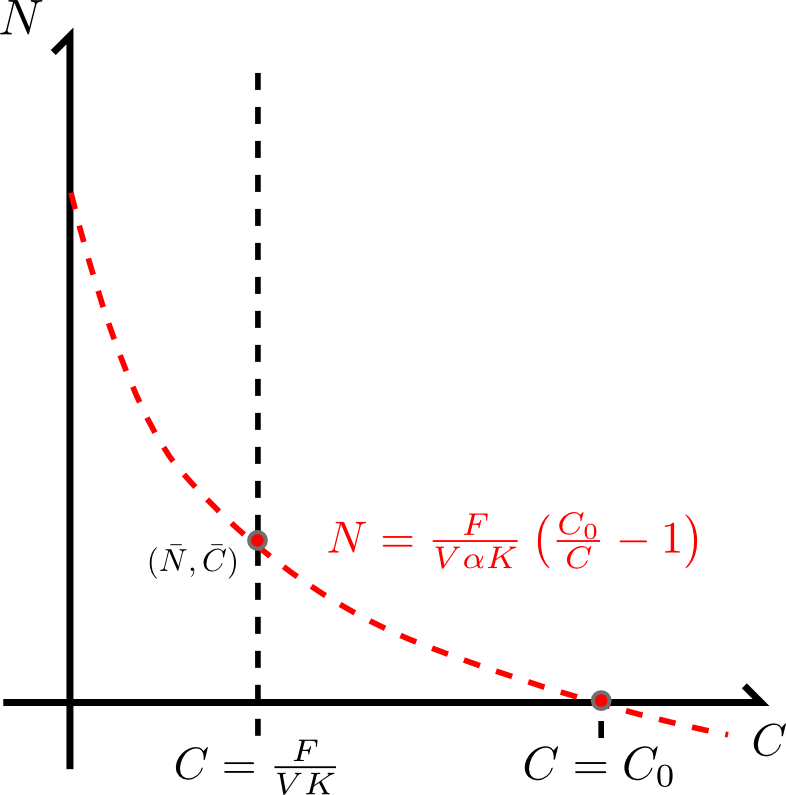
\includegraphics[width=1.0\textwidth]{../doc/images/drawing.png}
    \caption{\footnotesize The $\dot{C} = 0$ nullcline (dashed red) intersecting with the $\dot{N} = 0$ nullcline (dashed black).  The trivial and non-trivial steady-states $(0, C_0)$ and $(\bar{N}, \bar{C})$ are shown as red dots.}
  \end{figure}
  \end{column}
  \begin{column}{0.6\textwidth}
  \scriptsize
  By placing Eq.\ (3) inside Eq.\ (4), we can find the non-trivial steady-state, the intersection of null-clines:
  \begin{align}
    \bar{N}(\bar{C}) &= \frac{FC_0}{V \alpha K \bar{C}} - \frac{F}{V \alpha K}  \notag \\
    &= \frac{FC_0}{V \alpha K \frac{F}{VK}} - \frac{F}{V \alpha K} \notag \\
    &= \frac{C_0}{\alpha} - \frac{F}{V \alpha K} = \frac{1}{\alpha} \left( C_0 - \frac{F}{VK} \right).
  \end{align}
  The unknown parameters in Eq (5) are $\alpha$ and $K$.  We can find these parameters by fitting Eq (5) to the data by non-linear least squares fitting $\bar{N}_i$ at $F_i$ for $i = 1,\ldots,n$, where $n$ is the number of observations.
  \normalsize
  \end{column}
  \end{columns}
\end{frame}

%% frame =======================================================================
\begin{frame}
  \frametitle{The Data}
  \begin{figure}[H]
    \centering
      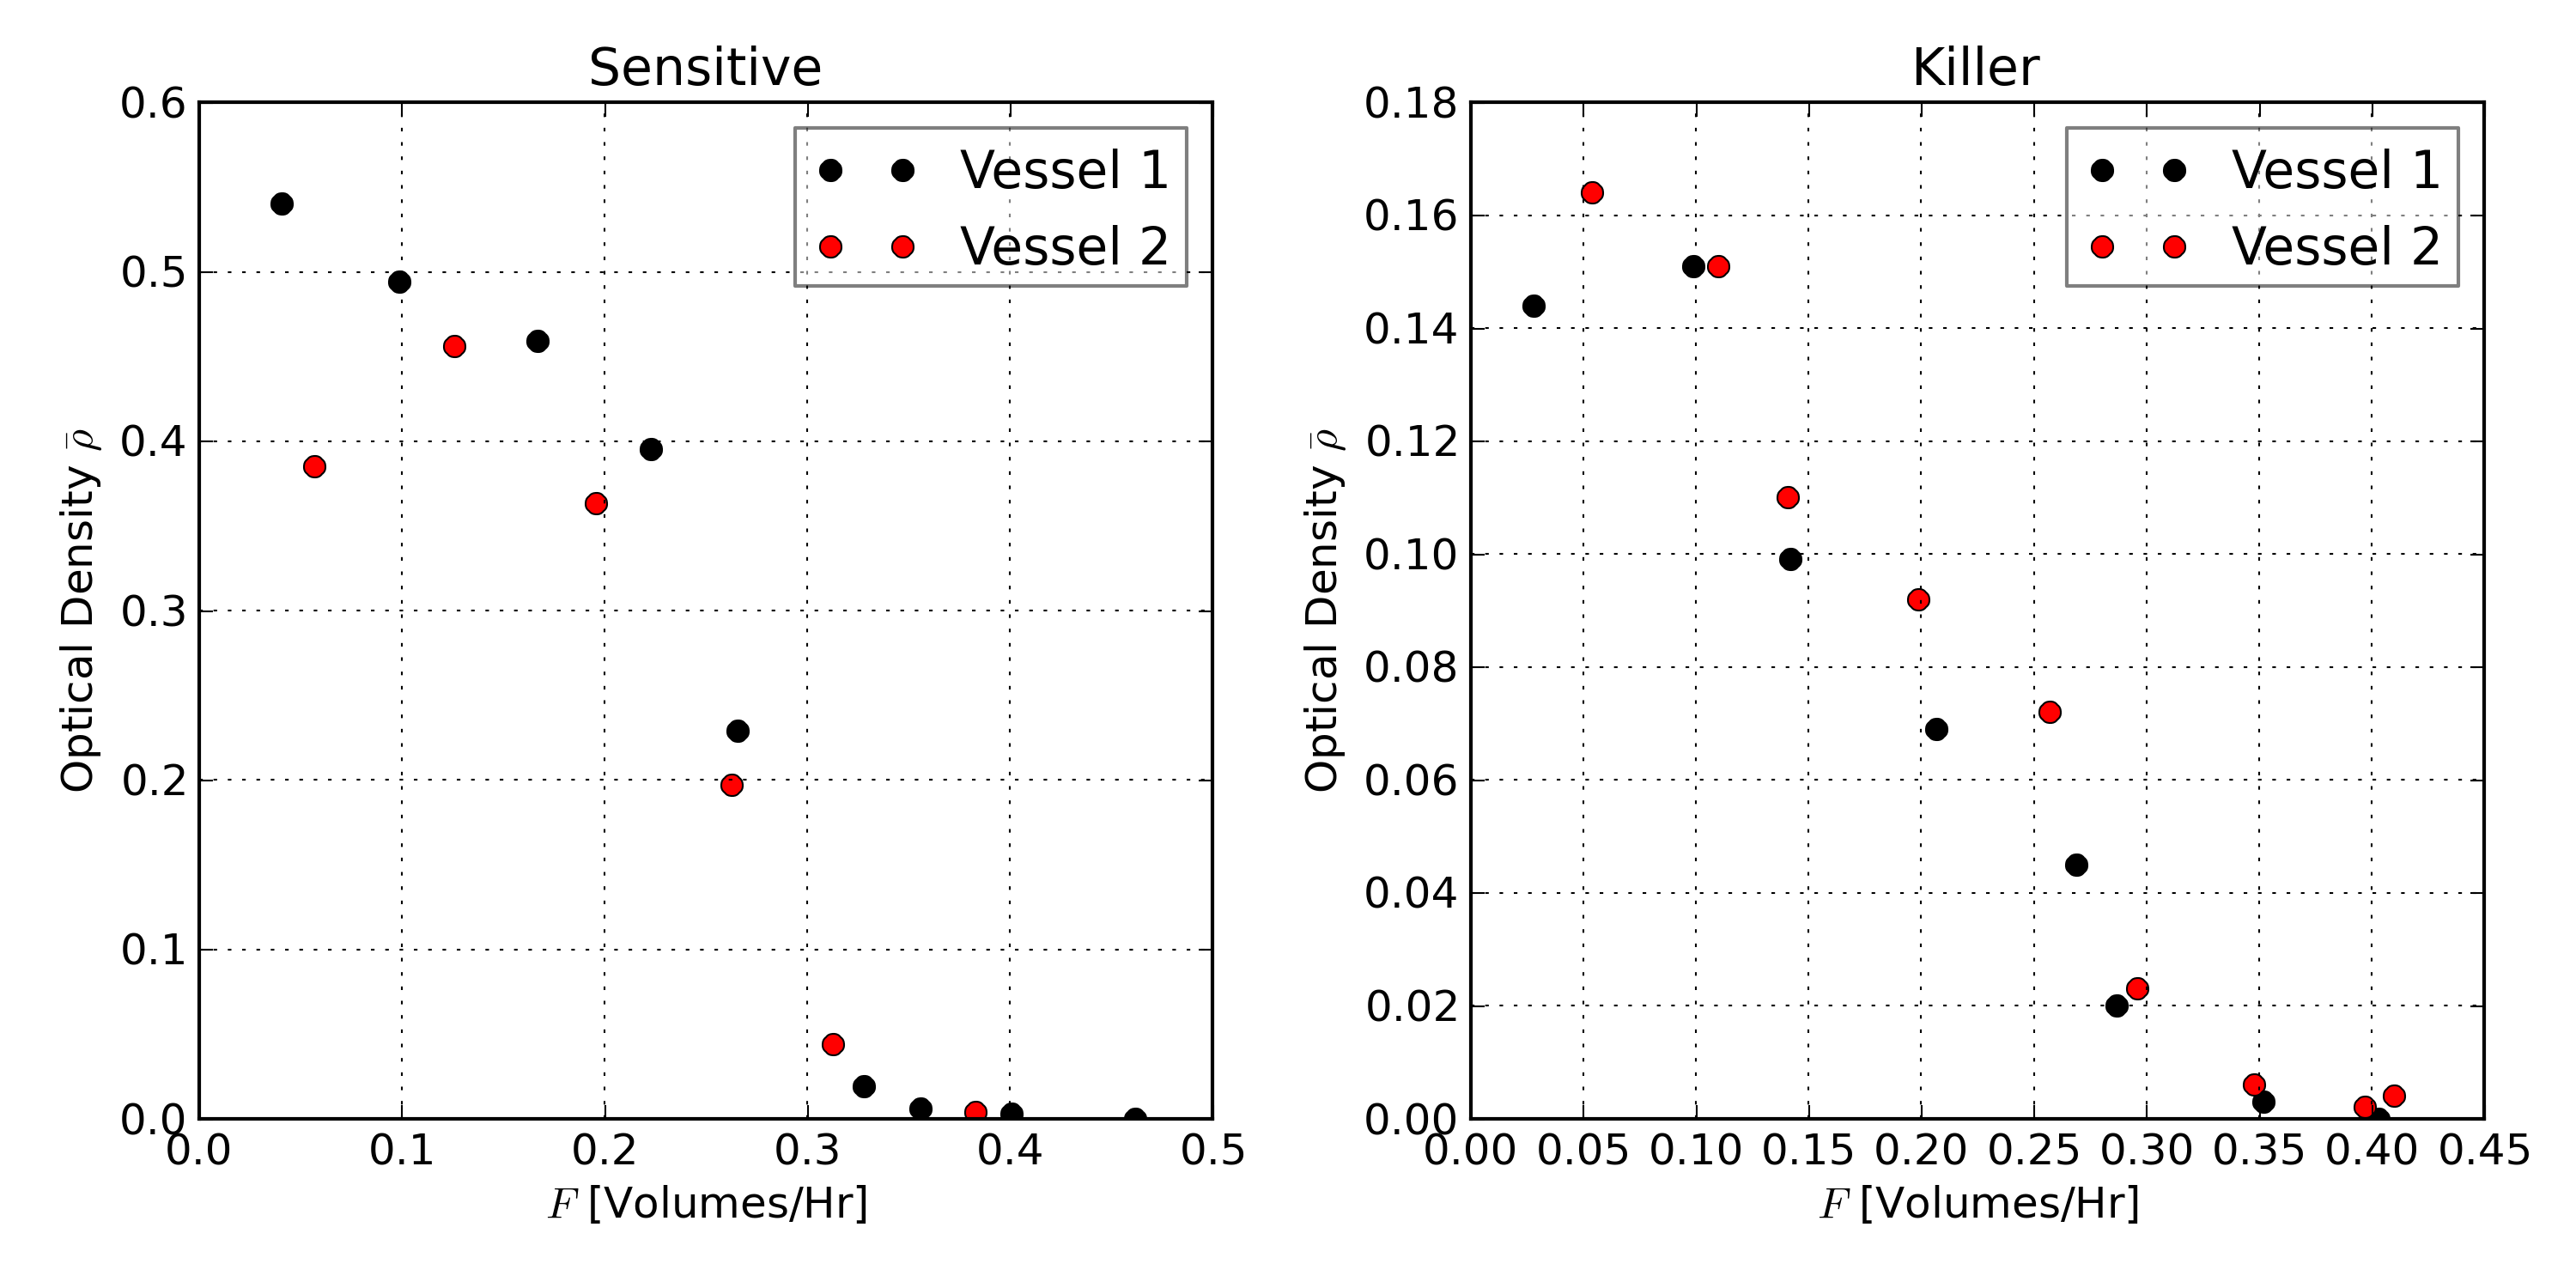
\includegraphics[width=1.0\textwidth]{../doc/images/data.png}
  \end{figure}
  $$C_0 = 0.02$$
\end{frame}

%% frame =======================================================================
\begin{frame}
  \frametitle{Eq.\ (5) Fit for Sensitive Yeast}
  \begin{columns}
  \begin{column}{0.4\textwidth}
  \begin{figure}[H]
    \centering
      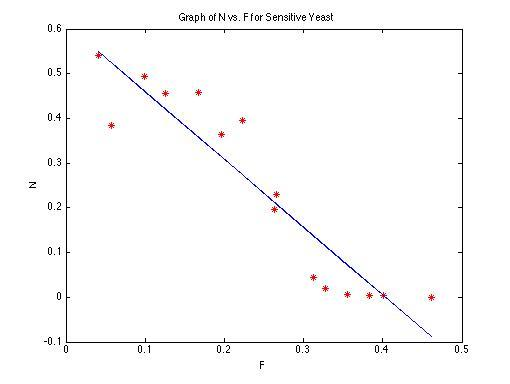
\includegraphics[width=1.0\textwidth]{../doc/images/sensitiveFit.jpg}
    \caption{\footnotesize Sensitive yeast $S$ steady-state best-fit line using Eq.\ (5).}
  \end{figure}
  \end{column}
  \begin{column}{0.6\textwidth}
  \footnotesize
  \begin{center}
  \begin{tabular}{l | c c c}
    & Estimates & SE & CI \\ 
    \hline
    $\alpha_S$ & 0.0325  & 0.0024 & (0.0255,  0.0399) \\
    $K_S$      & 20.1818 & 1.0802 & (16.9281, 23.4356) \\
  \end{tabular}
  \end{center}
  \normalsize
  The results on the left show that there may be a better fit to the data than Eq.\ (5).  Notice that elimination of the last few data points corresponding to high $F$ may be removed; this would reduce the standard error and hence provide a better estimate for $\alpha_L$ and $K_L$.
  \end{column}
  \end{columns}
\end{frame}

%% frame =======================================================================
\begin{frame}
  \frametitle{Eq.\ (5) Fit for Killer Yeast}
  \begin{columns}
  \begin{column}{0.4\textwidth}
  \begin{figure}[H]
    \centering
      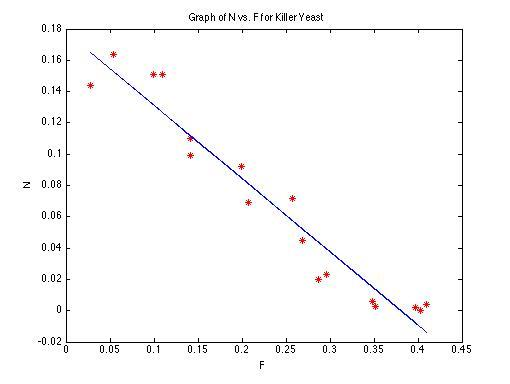
\includegraphics[width=1.0\textwidth]{../doc/images/killerFit.jpg}
    \caption{\footnotesize Killer yeast $L$ steady-state best-fit line using Eq.\ (5).}
  \end{figure}
  \end{column}
  \begin{column}{0.6\textwidth}
  \footnotesize
  \begin{center}
  \begin{tabular}{l | c c c}
    & Estimates & SE & CI \\ 
    \hline
    $\alpha_L$ & 0.1124  & 0.0053 & (0.0969,  0.1279) \\
    $K_L$      & 19.0288 & 0.6367 & (17.1526, 20.905) \\
  \end{tabular}
  \end{center}
  \normalsize
  The best-fit line on the left shows that steady-state data follows a fairly linear relationship with flow, and as such we can be confident our estimates for $\alpha_L$ and $K_L$ are correct.
  \end{column}
  \end{columns}
\end{frame}

%% frame =======================================================================
\begin{frame}
  \frametitle{What-If Scenario}
  Now that we have obtained estimates of the parameters for both the killer yeast $L$ and sensitive yeast $S$, ($\alpha_L$, $\alpha_S$ and $K_L$, $K_S$ respectively), we model a ``what if'' scenario whereby we place both species of yeast, sensitive and killer, into one chemostat.  The differential equations we use to solve this three-species model is
  \begin{align}
    \frac{dL}{dt} &= K_L CL - \frac{FL}{V}, \\
    \frac{dS}{dt} &= K_S CS - \frac{FS}{V} - \beta S L, \\
    \frac{dC}{dt} &= -\alpha_L K_L CL -\alpha_S K_S CS - \frac{FC}{V} + \frac{FC_0}{V}.
  \end{align}
\end{frame}

%% frame =======================================================================
\begin{frame}
  \frametitle{What-if Scenario}
  We can run the dynamic model (6), (7), and (8) to equilibrium.  By letting $\beta$ range from 0 to 0.5 (in units 1/time), and $F$ range from 0 to 0.5 (in units volume/time), we can run the model for each $\beta$ and $F$ to determine the regions in the $\beta$, $F$ plane where sensitive yeast $S$ overtakes the killer yeast $L$ and vice versa.
\end{frame}

%% frame =======================================================================
\begin{frame}
  \frametitle{What-if Scenario Results}
  \begin{figure}[H]
    \centering
      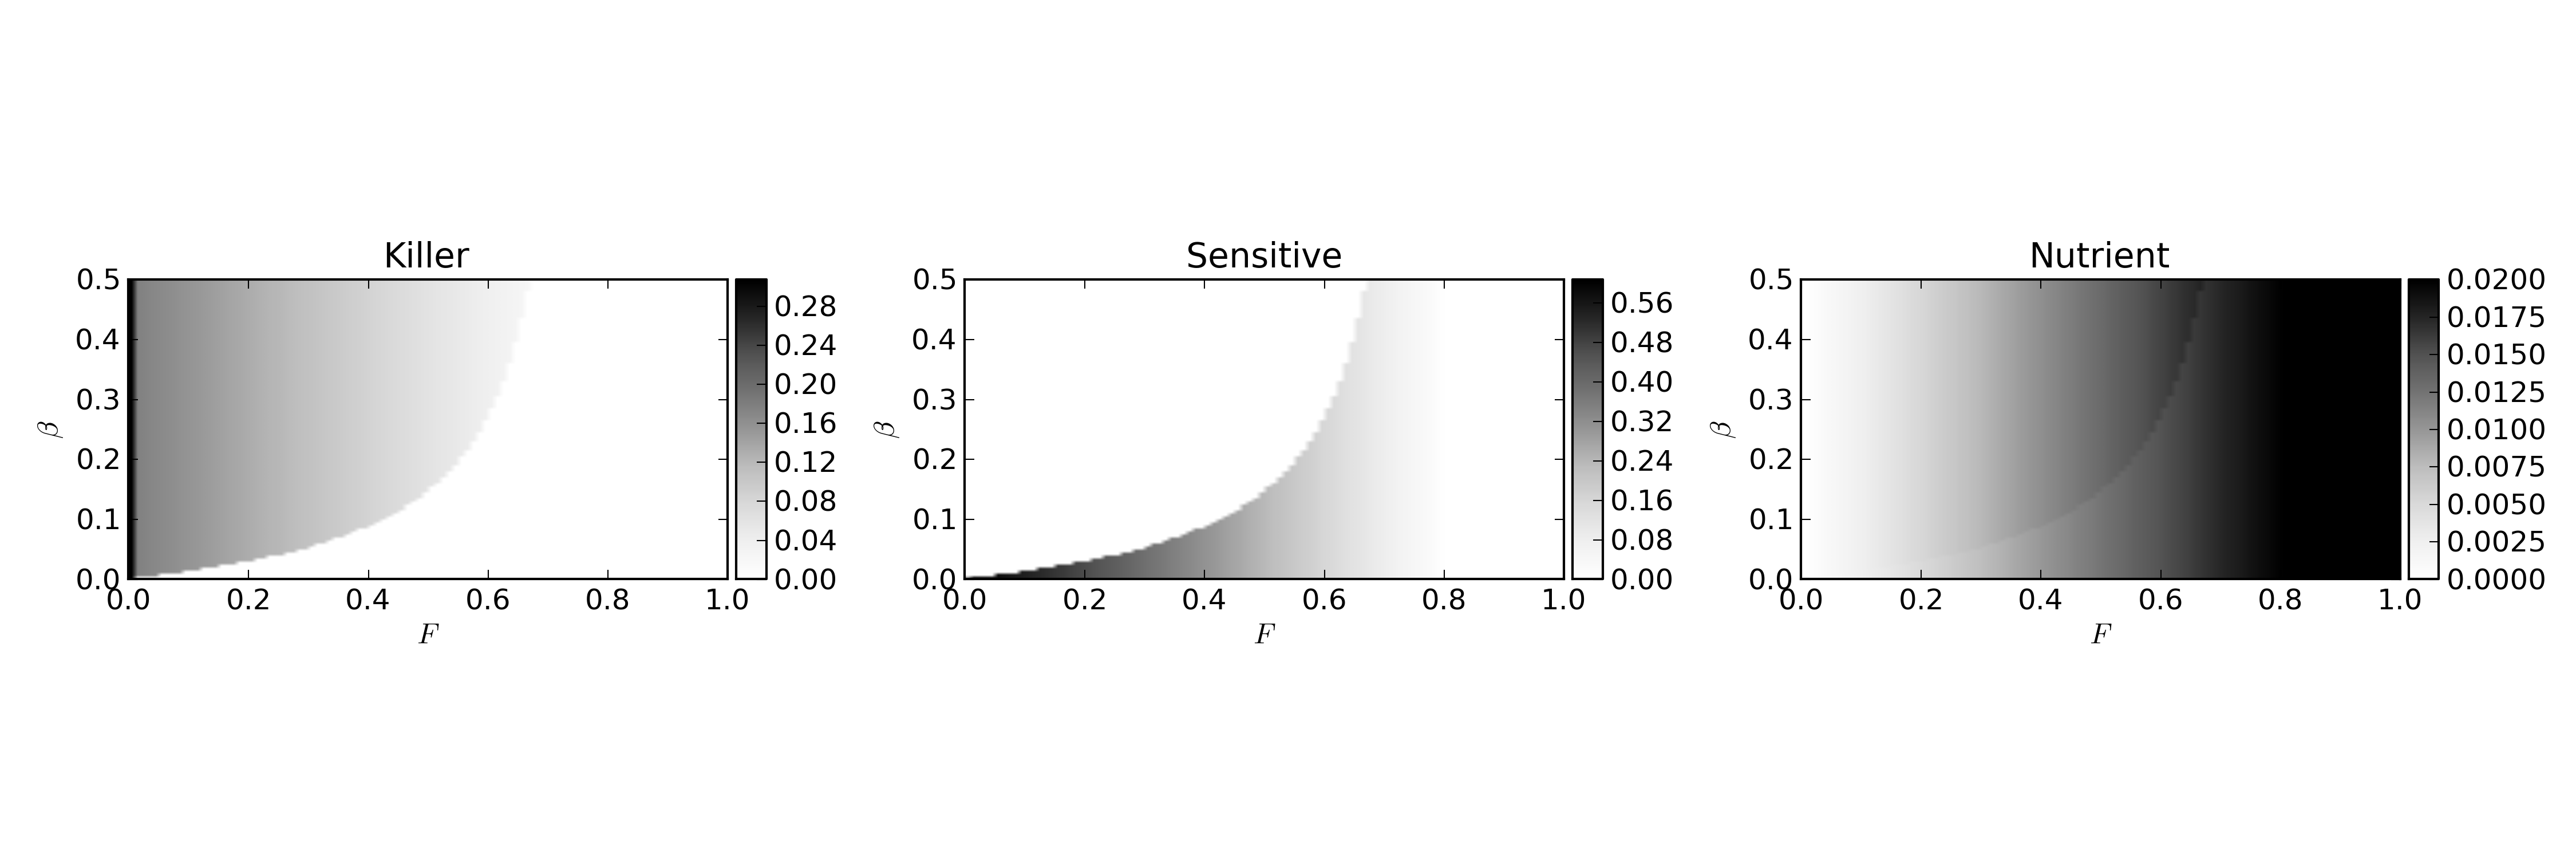
\includegraphics[width=1.0\textwidth]{../doc/images/sols.png}
    \caption{\footnotesize $250 \times 250$ steady-state optical density solution for killer yeast (left), sensitive yeast (middle) and nutrient (right) for a total run time of 40,000 hours.  Equations (6), (7), and (8) were solved with the Dormand-Prince numerical integration algorithm with an absolute tolerance of 1e-6, relative tolerance of 1e-6, and timestep $\Delta t$ of 500 hours.  The timestep was kept high due to the $250 \times 250 = 62,500$ simulations required to complete the figure.  In order to keep the total time to complete the simulation minimized, parallel processing was required.}
  \end{figure}  
\end{frame}

%% frame =======================================================================
\begin{frame}
  \frametitle{What-if Scenario Results}
  \begin{columns}
  \begin{column}{0.6\textwidth}
  \begin{figure}[H]
    \centering
      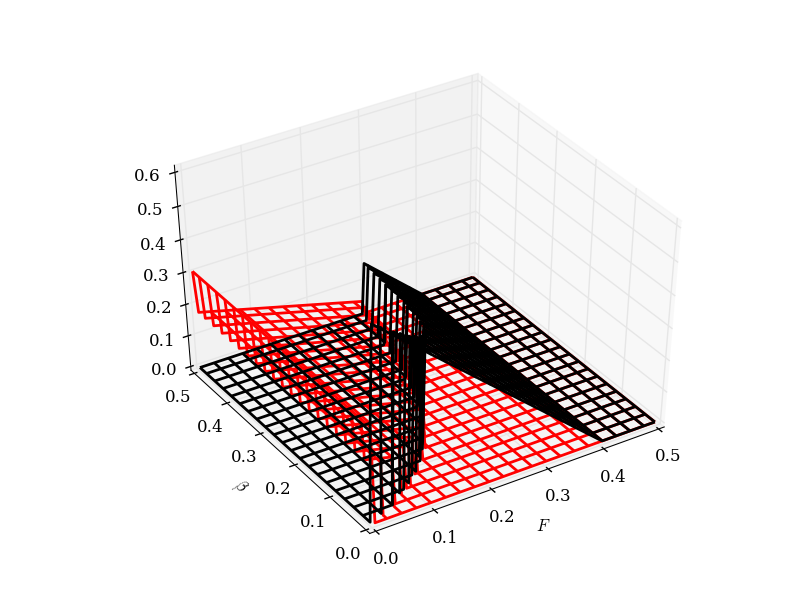
\includegraphics[width=1.0\textwidth]{../doc/images/3d.png}
    \caption{\footnotesize 3D solution depicting killer yeast (red) and sensitive yeast (black) steady-states.}
  \end{figure}
  \end{column}
  \begin{column}{0.4\textwidth}
  \footnotesize Notice that as $\beta$ increases the killer yeast dominates and sensitive yeast eventually dies off, while as $F$ increases the sensitive yeast dominates and the killer yeast eventually dies out.  The sensitive yeast are flushed from the container at around $F = 0.4$ volumes/hr.
  \normalsize
  \end{column}
  \end{columns}
\end{frame}

%% frame =======================================================================
\begin{frame}
  \frametitle{Questions?}
  \begin{figure}[H]
    \centering
      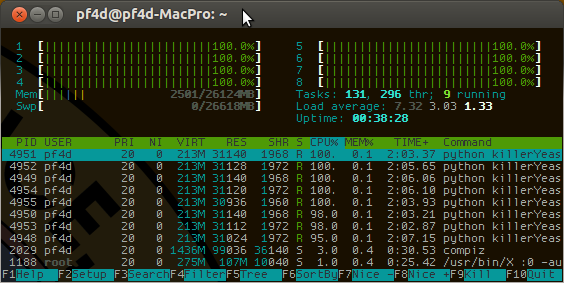
\includegraphics[width=1.0\textwidth]{images/cpuUse.png}
  \end{figure}

\end{frame}

\end{document}
